

\section{Information Flow Control} %mere konkret og teknisk
%Selvom jeg ikke kiggr på fx trafic analysis så er det vigtigt at nævne og påpege det ikkeer noget jeg løser
In the beginning of this chapter, the security properties confidentiality and integrity were mentioned which are major security goals for a system. If there is \emph{secure information flow} throughout the system, then confidentiality and integrity is achieved \cite{Hedin2011}. Secure information flow means that only authorized flow of information is allowed \cite{Denning1976}. There are two aspects to secure information flow; the reading of the information (confidentiality) and the writing of the information (integrity) \cite{Hedin2011}. 

\emph{Information Flow Control} is a \emph{security mechanism}\footnote{"A security mechanism is a method, tool, or procedure for enforcing a security policy" \cite{Bishop2004}} for achieving secure information flow.
Information Flow Control is a language-based security technique that can enforce defined \emph{security policies}\footnote{"A security policy is a statement of what is, and what is not, allowed." \cite{Bishop2004}} concerning confidentiality and integrity of data. It enables us to express where information may flow to and under what conditions. 

\subsection{Lattice model}\label{lattice}

By classifying information with \emph{security levels}, we can express where information may flow. Consider the following confidentiality policy; we classify \emph{secret} as secret information, and classify \emph{public} as public information. For the two security levels we express what information may flow where by classifying information with a security level, It holds that flow from public to public is allowed, public to secret is allowed, and secret to secret is allowed. For preserving confidentiality, flow from secret to public is under no circumstances allowed.  This can be expressed as \emph{public $\leq$ secret}, and we can formalize these flow constrains by means of a lattice\footnote{https://en.wikipedia.org/wiki/Lattice\_(order)} structure where information flows upwards shown in figure \ref{fig:lattice}a \cite{Smith}.


\begin{figure}[H]
	\centering
	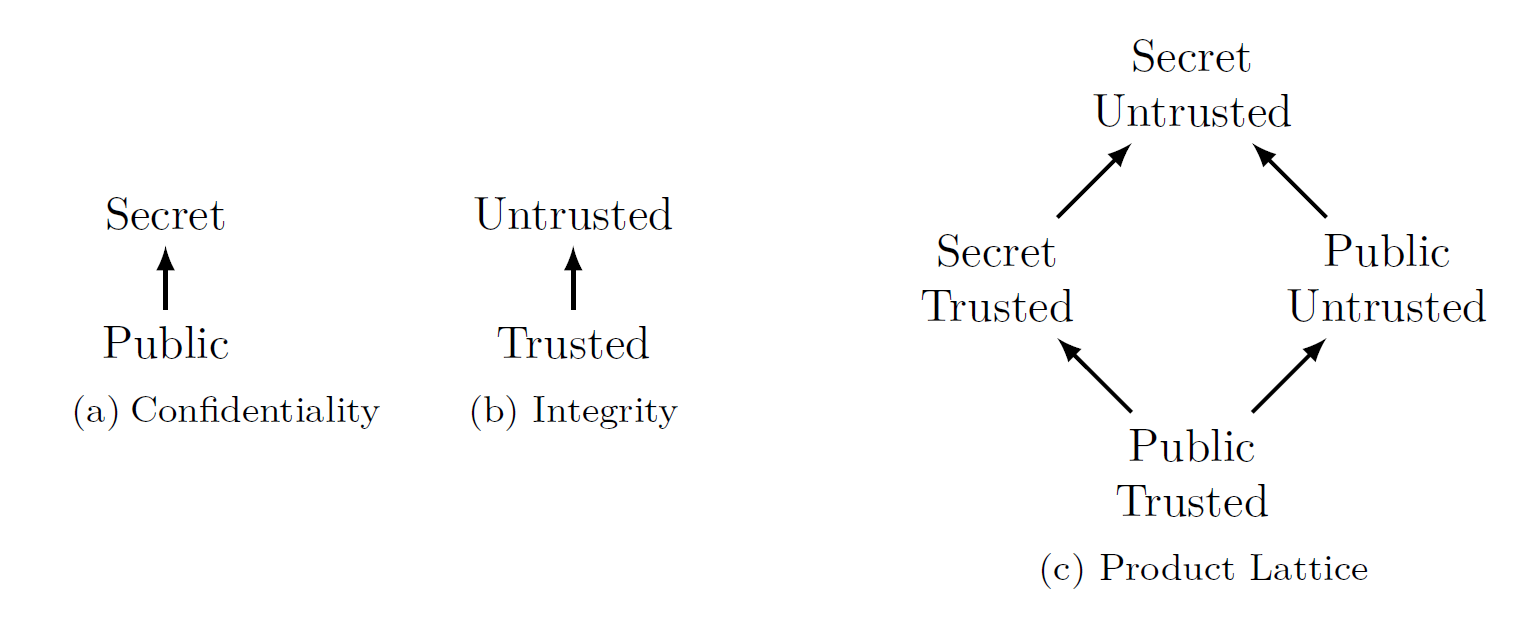
\includegraphics[width=12cm]{figures/lattice.png}
	\caption{ Lattice model for confidentiality and integrity \cite{Musard2014}}
	\label{fig:lattice}
\end{figure}

Likewise, a policy for integrity can be specified where information from an \emph{untrusted} source must not flow to information with a security level of \emph{trusted}, which is exactly the opposite of the confidentiality policy. Figure \ref{fig:lattice}b illustrates an integrity lattice. By combining the two we get a lattice show in figure \ref{fig:lattice}c.

\subsection{Explicit and implicit flow}\label{explicitimplicit}
The problem with mainstream programming languages is that they are unable to enforce defined policies such as the confidentiality and integrity policies described in the previous section. Consider the following flow:

\begin{lstlisting}
public = secret;
\end{lstlisting}

This is an \emph{explicit flow} since the \emph{secret} value is directly copied into the \emph{public} value, which obviously is a violation of the confidentiality policy and is an insecure flow of information \cite{Hedin2011}. 

Another example of insecure information flow is \emph{implicit flow}:

\begin{lstlisting}[language=ALGOL]
public = false;
if secret then public = true
\end{lstlisting}

In this example, the \emph{secret} value affects the control flow and some information is leaked about the \emph{secret} value. Hence this also violates the confidentiality policy. When secret values can affect the control flow there is an implicit flow \cite{Sabelfeld2003}.
%Security is equivalent to \emph{secure information flow}

\subsection{Covert channels} The explicit and implicit flows can also be considered as \emph{channels} that signal information \cite{Kashyap2011} \cite{Sabelfeld2003}. \emph{Covert channels} are channels that are not meant to signal information but somehow leaks information \cite{Kashyap2011}. The most prominent covert channels are: 
\begin{itemize}
	\item \emph{Implicit channels} leaks information through the path the program takes in the control flow.
	\item \emph{Termination channels} leaks information by considering if a program terminates.
	\item \emph{Timing channels} leaks information by considering when an action occurs or how much time a program takes.
\end{itemize}

Other channel are \emph{probabilistic channels}, \emph{resource exhaustion channels}, and \emph{power channels}. It is not necessarily all covert channels that are of concern and in the end depends on what is observable by an adversary \cite{Sabelfeld2003}.

\subsection{Noninterference}
Secure information flow can be expressed by the concept of \emph{noninterference}. The notion of noninterference is that someone observing the public input and output of a system and can pick the public input should not be able to learn anything about the secret input of the system. If the secret input interferes with the public output then there is information leak. The figure \ref{fig:noninterference} illustrates noninterference \cite{Hedin2011}.  

% The policies defined in section \ref{lattice} are noninterference policies \cite{Sabelfeld2003}. 


\begin{figure}[H]
	\centering
	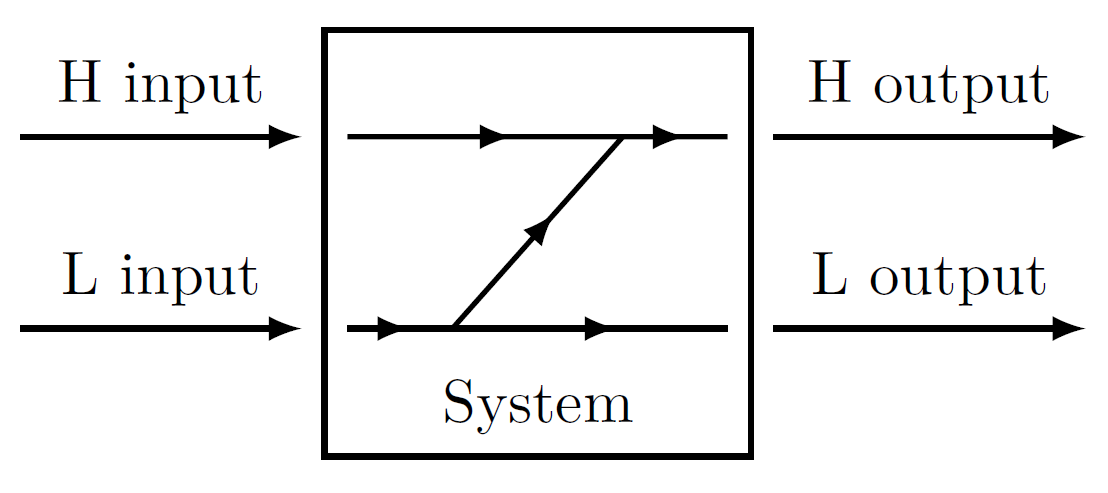
\includegraphics[width=8cm]{figures/noninterference2.png}
	\caption{ Noninterference \cite{Musard2014}}
	\label{fig:noninterference}
\end{figure}

The figure illustrates that the low confidentiality output \emph{L} (public) should be independent of the \emph{H input} (secret). In other words if a program is executed with fixed public input but with different secret input; then there should not be any changes to the public output \cite{Hedin2011}.


Depending on what an observer is capable of observing; different variations of noninterference can be expressed. Two of such variants are \emph{termination-insensitive} and \emph{termination-sensitive}.


\subparagraph{Termination-insensitive noninterference}

Termination-insensitive noninterference would guarantee that when a program terminates; the program's public output remains unaffected of the secret input. However it is possible to leak information through termination channels. By observing termination; 1 bit leaks can be achieved for each run of the program \cite{Hedin2011}:

\begin{lstlisting}
if (secret == public) then while (true) do skip done
\end{lstlisting}

If the program does terminate then the observer has learned that the secret is not equal to the public value hence 1 bit of information is leaked. 

%Save the argument of more than 1 bit leak to the discussion.

\subparagraph{Termination-sensitive noninterference}
The alternative is the termination-sensitive noninterference variant. The public output is independent of the secret input. Furthermore if the program is run with secret input \emph{s\textsubscript{1}} and it terminates; then the program run with secret input \emph{s\textsubscript{2}} would terminate as well. Hence if \emph{s\textsubscript{1}} did not terminate then \emph{s\textsubscript{2}} would not either \cite{Hedin2011}.

This variant of noninterference does not allow secret variables as guards in loops  and if-else-than statements as long as those in no way affect possible future \emph{L} output. This variant would be more restrictive and disallow flows as such \cite{Hedin2011}:

\begin{lstlisting}
while (secret == true) do ... done
\end{lstlisting}

\subsection{Declassification}
Noninterference is a very strict policy and not practical. Consider the classic example of a user logging into a system. It is unavoidable that a login attempt gives some information away about whether or not the password combination was valid. If the password is incorrect the login fails and partial information is given away. There is no problem with the above and is regarded as secure. Another example is sending encrypted data over an insecure channel; secret input is encrypted and the cipher text would then be sent over an insecure channel. However this goes against noninterference since the secret input clearly interferes with public output \cite{Hedin2011}.

Declassifying of information is necessary. Taking some specific information from a higher security class and changing it to a lower security classification is declassification. When declassifying information the following four dimensions needs to be addressed \cite{Sabelfeld2009}:

\begin{itemize}
	\item \emph{What} information should be declassified. We would like to specify what information is released.
	\item \emph{Who} can declassify the information. By specifying exactly who can release information it rules out that someone unspecified can make unintended leaks through declassification.
	\item \emph{Where} the information can flow. The dimension describes which security levels the declassified information may flow to and also where in the code the declassification occurs. 
	\item \emph{When} the declassification occurs. The release of information is only allowed relative to some even e.g. only after a purchase can a software key be released.
\end{itemize}



\subsubsection{Decentralized label model}\label{dlm}
\emph{Decentralized Label Model} allows us to define flow policies and address declassification of information in a program. A policy is defined by adding \emph{labels} to a value. A value can hold information for different \emph{principals} called \emph{owners}. A label \emph{L} specifies an \emph{owners} set \emph{owners(L)}. Each owner can allow a list of principals called readers \emph{readers(L,O)} that the information may be released to. \emph{Effective readers} are readers that all owners agree on the information can be released to and is essentially those where information can flow to. An example of a label is \textbf{\{\emph{o\textsubscript{1}}:\emph{r\textsubscript{1},r\textsubscript{2}}; \emph{o\textsubscript{2}}:\emph{r\textsubscript{2},r\textsubscript{3}}\}}; where  \emph{o\textsubscript{1}} and \emph{o\textsubscript{2}} are the different owners with their specified readers \cite{Myers1997}. The example \emph{L} has the following:

\[owners(L) = \{o_1, o_2\}\]
\[readers(L,o_1) = \{r_1, r_2\} \]
\[readers(L,o_2) = \{r_2, r_3\} \]
\[effectiveReaders(L) = \{r_2\} \]

Such labeling makes it possible for each owner to have an independent flow policy and give control of where the information may flow. Declassification is possible if the program detects it is running as the authority of one of the owners \cite{Myers1997} \cite{Myers1998}. This is known as the \emph{principal hierarchy} and can allow a principal to act for another principal.

%Apart from labels, there is one other important component to the DLM, namely the principal hierarchy, specified by a reflexive and transitive acts-for relationship. If Eve acts for Dave then Eve can do anything that Dave can. In the example above this means Eve can also read data with the label given above.

\subsection{Information-flow enforcement}
There exist two general techniques for enforcing secure information flow; \emph{static analysis} through e.g a type system, and \emph{dynamic analysis} through e.g. a monitor. Both techniques give the assurance of termination-insensitive noninterference \cite{Sabelfeld2010}. The static analysis have the advantage that it does not have the runtime overhead as the dynamic analysis while the dynamic analysis is more permissive \cite{Sabelfeld2010}. 


\subsubsection{Static enforcement}
Enforcement of information-flow through static analysis is done using type systems.
A simple type system is presented and shown in figure \ref{fig:typesystem}. 

\begin{figure}[H]
	\centering
	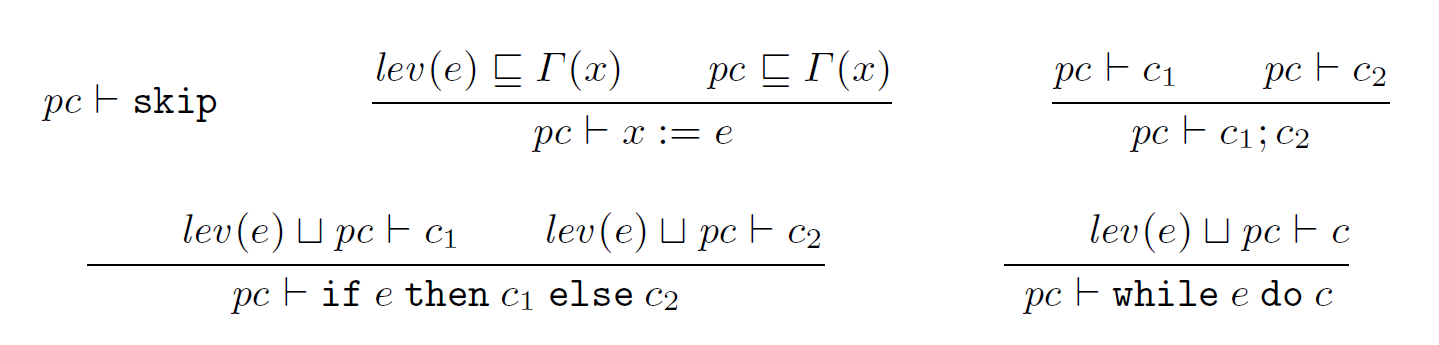
\includegraphics[width=12cm]{figures/securitytypesystem.png}
	\caption{ Typing rules \cite{Sabelfeld2010}}
	\label{fig:typesystem}
\end{figure}

We assume that the security lattice has the levels \emph{L} for low (public) and \emph{H} for high (secret). $\Gamma$ denotes a typing environment that takes a variable \emph{x} and maps it to a security level. The function \emph{lev(e)} takes an expression \emph{e} and returns a security level; if \emph{e} holds a high variable then \emph{H} is returned or else \emph{L} is returned. The security level of the context is kept tracked of by the program counter \emph{pc}. The typing judgment for commands is denoted by \emph{pc $\vdash$ c} \cite{Sabelfeld2010}.

The typing rule \emph{pc $\vdash$ x := e} is for assignment; it prevent assignment of a expression that holds a high variable to a low variable \cite{Sabelfeld2010}. Hence the explicit flow would be detected by the type system:

\begin{lstlisting}
low = high
\end{lstlisting}

Furthermore implicit flow are detectable through the program counter \emph{pc}. If there is a high guard then the \emph{pc} has the security level \emph{H} and would expect assignments of high variables hence preventing low assignments \cite{Sabelfeld2010}. The implicit flow would be detected by the typing system as well:

\begin{lstlisting}
if high then low = true else low = false
\end{lstlisting}


\subsubsection{Dynamic enforcement}
Dynamic analysis is provided with \emph{monitors}. Monitoring can only consider one path when running. This has led to the belief that the dynamic approach falls short compared to the static enforcement. However both dynamic enforcement and static enforcement achieve termination-insensitive noninterference hence they give the same security assurance \cite{Sabelfeld2010}. 

\begin{figure}[H]
	\centering
	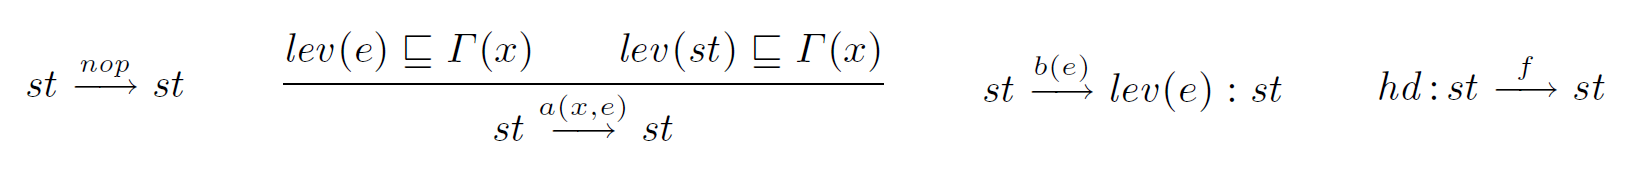
\includegraphics[width=12cm]{figures/monitoringrules.png}
	\caption{ Monitoring rules \cite{Sabelfeld2010}}
	\label{fig:monitoring}
\end{figure}

The figure \ref{fig:monitoring} shows monitoring rules for a monitor. Programs generates events and the monitor chooses to accept an event or block it by halting. Security levels are tracked by stack \emph{st} which is called a \emph{monitor configuration} and serves the same purpose as the program counter; keeping track of the current security context.  The monitor can execute following \emph{events} generated by the program: 

\begin{itemize}
	\item \emph{nop event:} signals a skip and the monitor always this event. It does not change the state of the monitor.
	\item \emph{assignment event a(x,e):} assigns the value of expression \emph{e} to variable \emph{x}. It does not change the state of the monitor but the monitor has the following two conditions:
	\begin{enumerate}
		\item \emph{lev}(\emph{e}) $\sqsubseteq$ $\Gamma(x)$: the expression \emph{e}'s security level is equal or lower than variable \emph{x}'s security level.
		\item \emph{lev}(\emph{st}) $\sqsubseteq$ $\Gamma(x)$: the highest security level in the stack is equal or lower than variable \emph{x}'s security level 
	\end{enumerate} 
	\item \emph{branching event b(e)}: branches on \emph{e} and changes the state of the monitor. The security level of \emph{e} is pushed on the stack.
	\item \emph{event f}: signals are loop or if-else statement has finished evaluating. The security level pushed to the stack \emph{st} would be popped when evaluation is finished.
\end{itemize}

The first condition for the assignment event prevents explicit flows, since whenever the program takes a step, the monitor must take a step; if the monitor cannot take a step, that halts the program. The second condition prevents implicit flows as such: 

\begin{lstlisting}
if high then low=true else low=false
\end{lstlisting}

The mechanism related to the branching event aids in preventing implicit flows by pushing the security level of \emph{st} to the stack. Now consider the following code: 

\begin{lstlisting}
if high then low=true else skip
\end{lstlisting}

If high is \emph{false} then the code would continue however if high is \emph{true} the execution would be stopped. Hence 1 bit would be leaked and is acceptable in context of termination-insensitive noninterference.

\section{Summary}
The background section introduces security properties necessary for a secure system. Several other security properties are described relevant for a secure messaging system which is relevant for the section \ref{evaluationofmatrix} where Matrix security is evaluated. This section also presented a description of the Signal Protocol necessary for the evaluation as well. Furthermore Matrix and its architecture was described and finally the basic concepts of Information-Flow Control was presented.


\section{Analysis of IFC Tools}
%Enforcing new session start every time a patient journal is sent. Could it be enforced with IFC?
% Tools issue: java sdk for matrix is beta and not fully implemented. 
% Best supported sdk is for javascript or python. Problem of running javascript code or python code with Paragon (java)
% Maybe better to use JSFlow instead 

% This chapter will present the criteria \emph{Survey of IFC tools and selection of tool}


Different Information-Flow Control tools were considered to be used in the case study. This section describes three of those tools; \emph{Jif}, \emph{Paragon} and \emph{JSFlow}. This section further justifies the selection of Paragon.

\subsection{Jif}

Jif is a Java based security-typed programming language that provides information flow control through static enforcement. Jif implements the Decentralized Label Model (DLM) described in section \ref{dlm}. Policies are defined conforming to the DLM. The policies are enforced at compile time by and Information-Flow Security type system with support for enforcement of dynamic policies at runtime. If a Jif program adheres to the specified policies the Jif compiler then compiles it to a secure Java program \cite{jifmanual}. 

Each variable in Jif has a DLM
policy associated with it. A policy
is
A policy is defined by labels and are associated with program variables. A policy can specify multiple principles that have readers or writers. A policy is defined as: 

\begin{lstlisting}[mathescape]
int {Alice$\rightarrow$Bob; Alice$\leftarrow$Bob} x;
\end{lstlisting}

The policy specifies two things; that first part with "$\rightarrow$" expresses \emph{Alice} controls the variable x and the variable can be read by \emph{Bob}, the second part with "$\leftarrow$ expresses that bob can write to it \cite{jifmanual}. 

The following code shows another example:

\begin{lstlisting}[mathescape]
int {Alice} x;
int {Alice$\rightarrow$Bob} y;
x = y; // OK
y = x; // BAD
\end{lstlisting}


Variable  \emph{x} has a policy that \emph{Alice} controls with no readers. The variable \emph{y} is owned by \emph{Alice} with \emph{Bob} being able to read hence the label is less restrictive than \emph{x}'s label. The compiler allows the \emph{x = y} since \emph{Bob} is specified as a reader for \emph{x}. However the expression \emph{y = x} is illegal since \emph{x} has a stronger policy than y and the explicit flow is caught \cite{jifmanual}.


A important feature for security-typed languages are declassification. Noninterference is too strict for practical programs thus it is necessary to declassify information at times. The following example has two variables with different labels. Variable \emph{x} is more restrictive than \emph{y}; that has \emph{Bob} as a reader. The example depicts an implicit flow: 

\begin{lstlisting}[mathescape]
void implicitFlow(){
int {Alice$\rightarrow$} x;
int {Alice$\rightarrow$Bob} y;
if (x == 1) { 
// pc has label {Alice$\rightarrow$}
y = 0; // BAD
}
}
\end{lstlisting}

When the code branches on the if statement the pc has the label \emph{\{Alice$\rightarrow$\}} and the expression \emph{y = 0} becomes illegal since it has the label \emph{\{Alice$\rightarrow$Bob\}} which is less restrictive than the label pc is holding. If for some reason we would want the expression to become valid we would have to declassify it:

\begin{lstlisting}[mathescape]
void declassificationExample() where authority(Alice) {
int{Alice$\rightarrow$} x;
int{Alice$\rightarrow$Bob} y;
// PC has label {}
if (x == 1) {
// PC has label {Alice$\rightarrow$}
declassify({Alice$\rightarrow$} to {Alice$\rightarrow$Bob}) {
y = 0; // OK
}
}
}
\end{lstlisting}

To be able to declassify it must be through the authority of the owner. This has to be specified at the method definition. When the code branches on the if statement the program counter \emph{pc} has the label \emph{\{Alice$\rightarrow$\}} which can then be declassified to a label as restrictive as \emph{y}'s label \cite{jifmanual} \cite{Srikant}.

Another interesting feature is dynamic labels. Jif provides a run-time library which compares labels at runtime using a syntax that resembles if-statements.
\begin{lstlisting}[mathescape]
void m(int{*lbl} i, label{} lbl) {
int{Alice$\rightarrow$} x;
if (lbl <= new label {Alice$\rightarrow$}) {
x = i; // OK, since {*lbl} <= {Alice$\rightarrow$}
}
else {
x = 0;
}
}
\end{lstlisting}

The parameter variable \emph{i} has the label held by the label \emph{lbl} which would be resolved at runtime. Since the variable \emph{x} has label \emph{\{Alice$\rightarrow$\}}, we can allow a flow to that variable as long it is less or equally restrictive. The static analysis of the program will pass and the program will be able to compile.  
%Dynamic label example


Other relevant features that Jif supports are label inference\footnote{http://www.cs.cornell.edu/jif/doc/jif-3.3.0/language.html\#inference} and parameterized classes\footnote{http://www.cs.cornell.edu/jif/doc/jif-3.3.0/language.html\#parameterized-classes}.
\subsection{Paragon}

Paragon is a programming language that extends Java with the ability to express security policies for data. Paragon has similar characteristics to Jif and essentially solving the same problem. Paragon takes a different approach to defining information flow policies; \emph{Paralocks} \cite{paralocks} \cite{paragonpaper}.
At the core, \emph{Paralocks} is based on the concepts \emph{actors} and \emph{locks} \cite{paralocks}. An actor is a user with some role. For information can flow to an actor there might be a condition that states; that the actor must be of a specific role. These conditions are represented by boolean variables \emph{locks} and can be modified throughout program execution. These locks are called \emph{parameterized locks} since they are parameterized over actors. Policies are specified by parameterized locks and \emph{actor polymorphism} allows us to reason about all actors \cite{paragonpaper}.


In Paragon policies are immutable and the following example shows how policies can be defined:

\begin{lstlisting}
public static final policy low  = { Object x: };
public static final policy high = { };
\end{lstlisting}

Policies for \emph{low} and \emph{high} can encoded in different ways. The encoding specifies the most liberal policy that anyone can see the data that has the policy of \emph{low}. The actor is any \emph{Object x} hence anyone can read. The encoding for \emph{high} is the most strict policy and specifies that actors so no one can see the data \cite{paragonprogramming}.

To support a simple declassification mechanism a lock would have to be introduced and the \emph{high} policy definition would have to be redefined:

\begin{lstlisting}
private lock Declassify;
public static final policy low  = { Object x: };
public static final policy high = { Object x: Declassify};
\end{lstlisting} 

The \emph{high} policy now specifies that information can only be read if the \emph{ declassify lock} is open. The following method can now allow declassification:

\begin{lstlisting}
public static ?low int declassify(?high int x){
open Declassify { return x; } 
}
\end{lstlisting} 

The method is a custom declassification method for variables with type \emph{int}. By using Java generics the same method could be used for any type. The \emph{declassify()} method takes a parameter that has the policy \emph{high} and returns the parameter with the lower policy \emph{low}. The method opens the lock hence allowing the value of \emph{x} to be read and returned. 
%Java generics is used to allow declassification of any type.

\begin{lstlisting}
publicVariable = declassify(secretVariable); // OK
\end{lstlisting} 


The example illustrates a simple declassify method however it can be called by anyone. To ensure that only those with the right authority can call it the example could easily be extended with another lock \cite{paralocks}. 

It is possible to support policies at runtime with locks \cite{paragonprogramming}. Suppose we have a customer who buys some software. The software keys should only be given when the customer has paid. We define the following:

\begin{lstlisting}
public static lock Paid;
?{customer: } String customerData
?{customer: Paid} String softwareKey
\end{lstlisting}

When the the customer's payment is processed the lock \emph{Paid} should only be open if the payment is successful. 

\begin{lstlisting}
public void processPayment() {
// customer pays for item
if (paymentSuccessful) { open Paid; } else { ... }
}
\end{lstlisting}

It is not possible for the compiler to learn the state of the lock \emph{Paid}. By using the lock in a conditional statement the lock will be checked at runtime \cite{paragonprogramming}.

\begin{lstlisting}
processPayment();
if (Paid) { customerData = softwareKey; } else { ... }
\end{lstlisting}   

Paragon is a powerful tool for Information-Flow Control and has an interesting policy language with support for expressive dynamic policies. Other relevant features in paragon are policy inference and Java generics.

\subsection{JSFlow}

JSFlow is a tool for tracking information flow in JavaScript web applications. This tool is not a programming language as the two previously described tool but a JavaScript interpreter that supports full non-strict ECMA-262 \cite{jsflowsite}. JSFlow enforces secure information flow through dynamic analysis and can detect explicit and implicit flows. JSFlow uses a program counter \emph{pc} to track the security context. JSFlow defines two built-in security levels; \emph{public} and \emph{secret}, it also supports custom security labels on values. JSFlow allows pure explicit flows by upgrading the security label of the variable being assigned to \cite{jsflowsite}:

\begin{lstlisting}
high = lbl(true);
low = high;
\end{lstlisting}

The variable \emph{high} is assigned a secret value denoted by the \emph{lbl} function. When \emph{high} is assigned to \emph{low} the security label is upgraded for low. JSFlow prevents implicit flow through \emph{no sensitive update} that under secret control disallows changes to security labels \cite{Hedin2014}:

\begin{lstlisting}
high = lbl(true);
if(high){
l = true;
}
\end{lstlisting}

The execution would halt for the above code since no sensitive update is allowed. 

As mentioned before security labels can be assigned to variables. In the following examples \emph{l}, \emph{m} and \emph{h} is defined with different labels.

\begin{lstlisting}
var l = lbl(10, 'low');
var m = lbl(15, 'mid');
var h = lbl(20, 'mid', 'high');
if(m === 15) {
h=m; // OK
l=m; // BAD
}
\end{lstlisting}

JSFlows uses a subset lattice hence \emph{m} can flow to \emph{h} since \emph{m}'s label is a subset of \emph{h}'s labels \cite{jsflowsite}. The assignment \emph{l=h} would halt since the \emph{m}'s labels is not a subset of \emph{l}'s labels.


JSFlow is an exciting tool for dynamic Information-Flow Control. However the JSFlow is still immature and does not support important features such as declassification.

\subsection{Selection of IFC tool}
The approach to selecting a tool is from a programmer's perspective with emphasis on choosing the right tool for developing rather than the tool that achieves the best security. The rationale behind this is that if the tool is too strict, it is impossible to write practical programs in it.
The selection of the tool is based on different parameters that falls into two categories; \emph{technical features} and \emph{soft parameters}. The technical parameters are related to features that are necessary for developing the prototype while the soft parameters considers other aspects such as documentation, flexibility and permissiveness.

The technical features are relevant for applying the tool. The tool must have the following features; 

\begin{itemize}
	\item \emph{Define policies:} It must be possible to express where information may flow.
	\item \emph{Declassification:} Noninterference is too strict and the ability to declassify information is necessary. 
	\item \emph{Policy inference:} The tool can automatically infer labels to avoid retyping labels.
	\item \emph{Support for external libraries:} An important feature since the tool should be applicable to a Matrix SDK library.
	\item \emph{Run-time label checking} to enforce dynamic labeling.
\end{itemize}

The soft parameters are indirectly related to the tool. It can be an overhead developing if the program is to strict hence \emph{permissiveness} is defined as a parameter. The parameter \emph{flexibility} covers the flexibility and restrictiveness of the tool; it should be uncomplicated and straightforward work with the policy language. The final soft parameter is \emph{documentation}.

The table below gives an overview of the three tools related to the parameters. 

\begin{table}[H]
	\hspace*{-1.2cm} 
	\centering
	\begin{tabular}{r|ccccccccc}
		&
		\rot{Defining policies} &
		\rot{Declassification} &
		\rot{Run-time label checking} &
		\rot{Policy inference} &
		\rot{Support for external libraries} &
		\rot{Documentation} &
		\rot{Flexibility} &
		\rot{Permissiveness}
		\\ \hline
		Jif     & X & X & X & X & X & X &   &    \\ 
		Paragon & X & X & X & X & X &   & X &    \\
		JSFlow  & X &   & X & x &   &   &   & X  \\ 
	\end{tabular}
	
	\caption{Comparison of IFC tools}
	\label{fig:toolcomparison}
\end{table}


% Not possible to use Matrix library with JSFlow because of missing support for libaries such as require (in node). Also overhead with configuring JSFlow to be the interpretor.


JSFlow is still an immature tool and lack support important features. JSFlow does currently provide support for use with external libraries. It also lacks a mechanism for declassification. JSFlow would have been an interesting tool because of the permissiveness that comes with dynamic enforcement but also since the main Matrix SDK is for Javascript. 

Jif and Paragon offer many of the same features with the fundamental difference being the policy language. The policy language of Paragon is expressive, flexible and intuitive. Paragon is less restrictive and more flexible regarding the policies it specifies \cite{paragonpaper}. The programming experience in Paragon is more as an extension to Java then a different programming language which is the experience you get when programming in Jif. Jif however has a more complete documentation and more code examples to showcase. 

Another important aspect is the support for external libraries. Matrix can be used through client SDK's hence support for external libraries is necessary. Both Jif and Paragon supports this by allowing interacting with external Java classes. Both languages must specify a signature for the external Java class. %This was an overhead in Jif and even though Paragon uses the same approach it was easier to manage in Paragon.

Based on the consideration and parameters Paragon has been selected as the tool used in the case study. 


\section{Summary}
In this chapter the Matrix security model has been evaluated. Matrix provides end-to-end encryption and uses the Double Ratchet algorithm by Signal. To achieve end-to-end security the endpoints need to be secured as well \cite{Sabelfeld2003} this leads us to the chapter's second part. The chapter analyzed information-flow control tools and justifies the selection of Paragon which the prototype is programmed in. 